\documentclass[11pt]{article}
\usepackage[margin=1in]{geometry}
\usepackage{amsmath,amssymb,amsthm}
\usepackage{graphicx}
\usepackage[hidelinks]{hyperref}

\newtheorem{theorem}{Theorem}
\newtheorem{proposition}[theorem]{Proposition}
\newtheorem{corollary}[theorem]{Corollary}

\newcommand{\PP}{\mathcal P}
\newcommand{\BB}{\mathcal B}
\newcommand{\Nat}{\mathbb N}
\newcommand{\Rat}{\mathbb Q}
\newcommand{\Real}{\mathbb R}
\newcommand{\Span}{\operatorname{span}}

\begin{document}

\begin{center}
{\Large A fixed-representative partial reduction for Question 1 of arXiv:1912.03994}

\medskip
{\small Run \texttt{fa\_banach\_001}; source arXiv:1912.03994}
\end{center}

\section*{Status}

\textbf{corrected partial result.}

Cuth--Dolezal--Doucha--Kurka ask whether there is a continuous map
\(\Phi:\PP_\infty\to\BB\) such that \(X_\mu\) is linearly isometric to
\(X_{\Phi(\mu)}\) for every \(\mu\in\PP_\infty\). This packet gives a
positive answer on every stratum where a real-linearly independent dense
representative sequence is fixed in advance.

The previous version of this packet used rational linear independence.  The
audit of 21 June 2026 shows that this is not sufficient: membership in
\(\BB\) requires independence after passing to the real extension of the
pseudonorm.  That older packet is preserved in
\texttt{history/previous\_fixed\_representative\_packet\_rational\_independence\_flawed\_2026\_06\_16/}.

\section*{Source Questions}

The relevant source questions appear in arXiv:1912.03994, pages 20--21.

\begin{center}
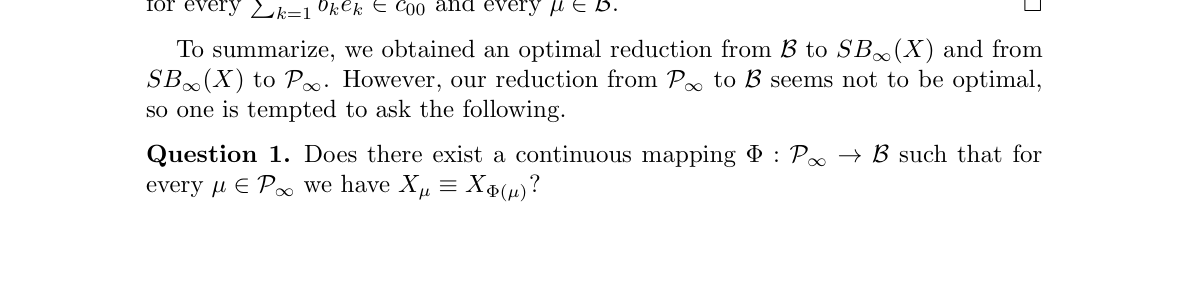
\includegraphics[width=0.95\linewidth]{figures/open_problem_crop_page20.png}

\medskip
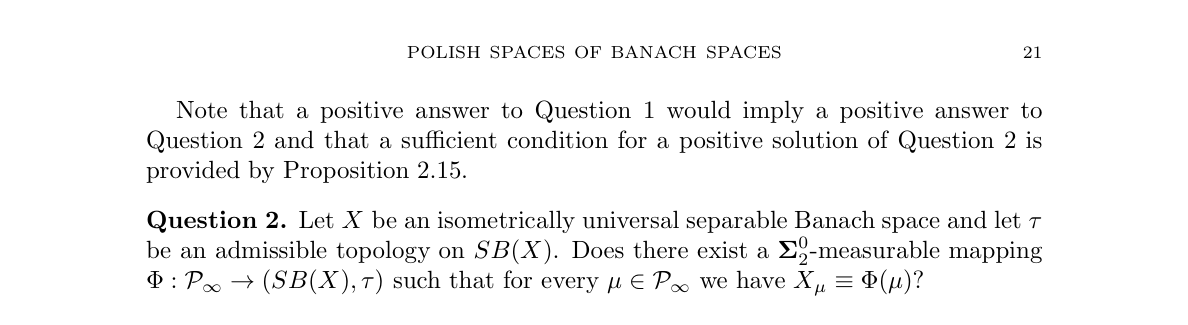
\includegraphics[width=0.95\linewidth]{figures/open_problem_crop_page21.png}
\end{center}

Question 1 asks for a continuous reduction \(\PP_\infty\to\BB\). Question 2
asks for the corresponding \(\boldsymbol{\Sigma}^0_2\)-measurable reduction
from \(\PP_\infty\) to \(SB(X)\) with an admissible topology.

\section*{Definitions}

Let \(V\) be the rational vector space with basis \((e_n)_{n\in\Nat}\), as in
the source paper. For \(\mu\in\PP\), write \(X_\mu\) for the completion of
\((c_{00},\mu)\) modulo its null space, and write \([v]_\mu\) for the image of
\(v\in V\) in \(X_\mu\).

Fix a strictly increasing sequence \(s=(s_j)_{j\ge1}\) in \(\Nat\). Let
\(\PP_s^{\mathrm{ind}}\subseteq\PP_\infty\) be the class of all \(\mu\)
such that:
\begin{enumerate}
\item for every \(m\in\Nat\),
\[
\inf_{\sum_{j=1}^m |a_j|^2=1}
\mu\Big(\sum_{j=1}^m a_j e_{s_j}\Big)>0,
\qquad a_j\in\Real,
\]
so the vectors \([e_{s_j}]_\mu\) are real-linearly independent;
\item the closed linear span of \(\{[e_{s_j}]_\mu:j\ge1\}\) is \(X_\mu\).
\end{enumerate}

\section*{Why the old rational condition was false}

The rational test is too weak.  For example, define on real \(c_{00}\)
\[
\mu(x)=|x_1-\sqrt2\,x_2|+\sum_{n=3}^\infty |x_n|.
\]
Its restriction to the rational vector space is positive on every nonzero
rational vector, but the real vector \(\sqrt2 e_1+e_2\) is \(\mu\)-null.
Thus the rational condition can hold while the real extension is not a norm.
This is exactly the gap repaired in the theorem below.

\section*{Proof Intuition}

The source paper already gives a \(\boldsymbol{\Sigma}^0_2\)-measurable
reduction by choosing, for each \(\mu\), the first coordinates that remain
linearly independent in \(X_\mu\). The discontinuity can only enter through
that coordinate-selection step. If the representative coordinates are fixed
beforehand, no selection remains: the output norm is just the restriction of
\(\mu\) to that fixed subsequence. Continuity is then immediate from the
coordinate topology on \(\PP\).

\section*{Theorem}

\begin{theorem}
For every strictly increasing sequence \(s=(s_j)\) in \(\Nat\), the formula
\[
\Phi_s(\mu)\Big(\sum_{j=1}^m a_j e_j\Big)
 =
\mu\Big(\sum_{j=1}^m a_j e_{s_j}\Big),
\qquad a_j\in\Rat,
\]
defines a continuous map \(\Phi_s:\PP_s^{\mathrm{ind}}\to\BB\), where
\(\PP_s^{\mathrm{ind}}\) has the
relative topology inherited from \(\PP_\infty\). Moreover
\[
X_{\Phi_s(\mu)}\equiv X_\mu
\]
linearly isometrically for every \(\mu\in\PP_s^{\mathrm{ind}}\).
\end{theorem}

\begin{proof}
Fix \(s\) and \(\mu\in\PP_s^{\mathrm{ind}}\). The formula defines a pseudonorm on \(V\)
because it is the pullback of the pseudonorm \(\mu\) under the fixed rational
linear injection \(T_s(e_j)=e_{s_j}\). The first defining property of
\(\PP_s^{\mathrm{ind}}\) says that no nonzero real vector of \(c_{00}\) is
sent to a \(\mu\)-null vector; hence the real extension of
\(\Phi_s(\mu)\) is a norm and \(\Phi_s(\mu)\in\BB\).

For continuity, let \(v=\sum_{j=1}^m a_j e_j\in V\). Then
\[
\Phi_s(\mu)(v)=\mu(T_s v).
\]
Since \(T_s v\in V\) is fixed, the map \(\mu\mapsto \mu(T_s v)\) is one of
the coordinate maps defining the topology of \(\PP\). Therefore every
coordinate of \(\Phi_s\) is continuous, which is precisely continuity as a map
into \(\BB\subseteq\PP\).

Finally define \(J_\mu:V\to X_\mu\) by \(J_\mu(e_j)=[e_{s_j}]_\mu\). For
every \(v\in V\),
\[
\|J_\mu v\|_{X_\mu}=\Phi_s(\mu)(v).
\]
Thus \(J_\mu\) descends to an isometric embedding of \(X_{\Phi_s(\mu)}\) into
\(X_\mu\). Its range contains the span of \(\{[e_{s_j}]_\mu:j\ge1\}\), which
is dense in \(X_\mu\) by the second defining property of \(\PP_s\). Hence the
extension of \(J_\mu\) is onto and is a linear isometry.
\end{proof}

\begin{corollary}
Let \(A\subseteq\Nat\) have infinite complement \(S=\{s_1<s_2<\cdots\}\). On
the stratum of all \(\mu\in\PP_\infty\) for which the coordinates
\(\{e_i:i\in A\}\) vanish and the quotient vectors
\(\{[e_{s_j}]_\mu:j\ge1\}\) are real-linearly independent, Question 1 has a
positive answer via \(\Phi_s\).
\end{corollary}

\begin{proof}
Under the stated hypotheses, every coordinate outside \(S\) is zero in the
quotient and every coordinate inside \(S\) belongs to the fixed representative
sequence. Hence the span of \([e_{s_j}]_\mu\) is dense in \(X_\mu\), and the
theorem applies.
\end{proof}

\section*{Relation to Question 2}

The companion full packet
\texttt{solutions/full/1912.03994\_question2\_sigma2\_dual\_ball\_parametrization/}
records the stronger 21 June 2026 audit result: a candidate full positive
answer to Question 2 on all pseudonorms.  The present packet is kept only as
the corrected fixed-stratum partial result for Question 1.

\section*{Verification and Limitations}

The proof is purely formal and uses only the definitions of the source coding
spaces. It does not solve the global problem because it assumes that the
representative sequence \(s\) is fixed on the whole domain. Thus the remaining
obstruction is precisely the source paper's global selection problem: choosing
such an independent dense sequence continuously as \(\mu\) varies over all of
\(\PP_\infty\).

The 21 June 2026 audit found no later resolution of Question 1.  It also
identified the rational-independence flaw above and supplied the corrected
real-independence formulation used here.

\section*{References}

\begin{thebibliography}{9}

\bibitem{CDDK}
M. Cuth, M. Dolezal, M. Doucha, and O. Kurka,
\emph{Polish spaces of Banach spaces},
arXiv:1912.03994.

\bibitem{CDDK2}
M. Cuth, M. Dolezal, M. Doucha, and O. Kurka,
\emph{Polish spaces of Banach spaces. Complexity of isometry and isomorphism classes},
arXiv:2204.06834.

\end{thebibliography}

\end{document}
